\documentclass[12pt]{article}

%%%%%%%%%%%%%%%%%%%%%%%%%%%%%%%%%%%%%%%%%%%%%%%%%%%%%%%%%%%%%%%%%%%%%%%%%%%%%%%%
%                           Package preset for homework
%%%%%%%%%%%%%%%%%%%%%%%%%%%%%%%%%%%%%%%%%%%%%%%%%%%%%%%%%%%%%%%%%%%%%%%%%%%%%%%%
% Miscellaneous
\usepackage[margin=1in]{geometry}
\usepackage[utf8]{inputenc}
\usepackage{indentfirst}
\usepackage{blindtext}
\usepackage{graphicx}
\usepackage{xr-hyper}
\usepackage{hyperref}
\usepackage{enumitem}
\usepackage{color}
\usepackage{float}
% Math
\usepackage{latexsym}
\usepackage{amsfonts}
\usepackage{amssymb}
\usepackage{amsmath}
\usepackage{commath}
\usepackage{amsthm}
\usepackage{bbold}
\usepackage{bm}
% Physics
\usepackage{physics}
\usepackage{siunitx}
% Code typesetting
\usepackage{listings}
% Citation
\usepackage[authoryear]{natbib}
\usepackage{appendix}
\usepackage[capitalize]{cleveref}
% Title & name
\title{Homework}
\author{Tien Vo}
\date{\today}


%%%%%%%%%%%%%%%%%%%%%%%%%%%%%%%%%%%%%%%%%%%%%%%%%%%%%%%%%%%%%%%%%%%%%%%%%%%%%%%%
%                   User-defined commands and environments
%%%%%%%%%%%%%%%%%%%%%%%%%%%%%%%%%%%%%%%%%%%%%%%%%%%%%%%%%%%%%%%%%%%%%%%%%%%%%%%%
%%% Misc
\sisetup{load-configurations=abbreviations}
\newcommand{\due}[1]{\date{Due: #1}}
\newcommand{\hint}{\textit{Hint}}
\let\oldt\t
\renewcommand{\t}[1]{\text{#1}}

%%% Bold sets & abbrv
\newcommand{\N}{\mathbb{N}}
\newcommand{\Z}{\mathbb{Z}}
\newcommand{\R}{\mathbb{R}}
\newcommand{\Q}{\mathbb{Q}}
\let\oldP\P
\renewcommand{\P}{\mathbb{P}}
\newcommand{\LL}{\mathcal{L}}
\newcommand{\FF}{\mathcal{F}}
\newcommand{\HH}{\mathcal{H}}
\newcommand{\NN}{\mathcal{N}}
\newcommand{\ZZ}{\mathcal{Z}}
\newcommand{\RN}[1]{\textup{\uppercase\expandafter{\romannumeral#1}}}
\newcommand{\ua}{\uparrow}
\newcommand{\da}{\downarrow}

%%% Unit vectors
\newcommand{\xhat}{\vb{\hat{x}}}
\newcommand{\yhat}{\vb{\hat{y}}}
\newcommand{\zhat}{\vb{\hat{z}}}
\newcommand{\nhat}{\vb{\hat{n}}}
\newcommand{\rhat}{\vb{\hat{r}}}
\newcommand{\phihat}{\bm{\hat{\phi}}}
\newcommand{\thetahat}{\bm{\hat{\theta}}}

%%% Other math stuff
\providecommand{\units}[1]{\,\ensuremath{\mathrm{#1}}\xspace}
% Set new style for problem
\newtheoremstyle{problemstyle}  % <name>
        {10pt}                   % <space above>
        {10pt}                   % <space below>
        {\normalfont}           % <body font>
        {}                      % <indent amount}
        {\bfseries\itshape}     % <theorem head font>
        {\normalfont\bfseries:} % <punctuation after theorem head>
        {.5em}                  % <space after theorem head>
        {}                      % <theorem head spec (can be left empty, 
                                % meaning `normal')>

% Set problem environment
\theoremstyle{problemstyle}
\newtheorem{problemenv}{Problem}[section]
\newenvironment{problem}[1]{%
  \renewcommand\theproblemenv{#1}%
  \problemenv
}{\endproblemenv}
% Set lemma environment
\newenvironment{lemma}[2][Lemma]{\begin{trivlist}
\item[\hskip \labelsep {\bfseries #1}\hskip \labelsep {\bfseries #2.}]}{\end{trivlist}}
% Set solution environment
\newenvironment{solution}{
    \begin{proof}[Solution]$ $\par\nobreak\ignorespaces
}{\end{proof}}
\numberwithin{equation}{problemenv}

%%% Page format
\setlength{\parindent}{0.5cm}
\setlength{\oddsidemargin}{0in}
\setlength{\textwidth}{6.5in}
\setlength{\textheight}{8.8in}
\setlength{\topmargin}{0in}
\setlength{\headheight}{18pt}

%%% Code environments
\definecolor{dkgreen}{rgb}{0,0.6,0}
\definecolor{gray}{rgb}{0.5,0.5,0.5}
\definecolor{mauve}{rgb}{0.58,0,0.82}
\lstset{frame=tb,
  language=Python,
  aboveskip=3mm,
  belowskip=3mm,
  showstringspaces=false,
  columns=flexible,
  basicstyle={\small\ttfamily},
  numbers=none,
  numberstyle=\tiny\color{gray},
  keywordstyle=\color{blue},
  commentstyle=\color{dkgreen},
  stringstyle=\color{mauve},
  breaklines=true,
  breakatwhitespace=true,
  tabsize=4
}
\lstset{
  language=Mathematica,
  numbers=left,
  numberstyle=\tiny\color{gray},
  numbersep=5pt,
  breaklines=true,
  captionpos={t},
  frame={lines},
  rulecolor=\color{black},
  framerule=0.5pt,
  columns=flexible,
  tabsize=2
}


\title{Homework 1: Astr 5140 (Fall 2021)}

\begin{document}

\maketitle


\begin{problem}{1}[Maxwellian distribution]

The most often used particle distribution in plasma physics is the drifting
Maxwellian separate parallel and perpendicular temperature
\begin{equation}\label{p1:3d_gaussian}
    f(\vb{v})=Ae^{-\frac{m}{2}\qty(
        \frac{(v_x-u_x)^2}{T_\perp}+
        \frac{(v_y-u_y)^2}{T_\perp}+
        \frac{(v_z-u_z)^2}{T_\|}
    )}
\end{equation}
where $\vb{u}$ is the drift velocity (fluid velocity), $\vb{v}$ is the
individual particle's velocity, and
\begin{equation}
    A=n\qty(\frac{m}{2\pi T_\perp})\qty(\frac{m}{2\pi T_\|})^{1/2} 
\end{equation}

(a) Show that
\begin{equation}
    \int_{-\infty}^\infty f(\vb{v})=n  
\end{equation}
\textit{Hint}: Substitute the variable $\vb{w}=\vb{v}-\vb{u}$. Do the 
integration for one dimension, then deduce the result for the other two 
dimension.

(b) Show that:
\begin{equation}\label{p1b:show}
    \int_{-\infty}^\infty\vb{v}f(\vb{v})=n\vb{u} 
\end{equation}
\textit{Hint}: Use symmetry arguments (e.g. the odd functions integrate to 0) to
avoid carrying out the integration. Be succint. Carry out the integration for
one direction and deduce the result for the other directions.

(c) Show that:
\begin{equation}
    \int_{-\infty}^\infty \vb{v}\vb{v}f(\vb{v})=n\vb{u}\vb{u}+\frac{n\vb{T}}{m} 
\end{equation}
where $\vb{T}=\text{diag}\qty(T_\perp,T_\perp,T_\|)$. \textit{Hint}: Solve one
diagonal term, for example $v_xv_x$, and one off-diagonal term, for example
$v_xv_y$. Deduce the results for the remaining terms. Again, use symmetry
arguments where possible.

(d) Sketch $f$ versus $v_x$ by hand.


\begin{solution}
    (a) Note from \eqref{p1:3d_gaussian} that
    $f(\vb{v})=n\prod_{i\in\qty{x,y,z}}g(v_i)$ where
    \begin{equation}\label{p1:g}
        g(v_i)=\sqrt{\frac{m}{2\pi
        T_i}}\exp\qty[-\frac{m(v_i-u_i)^2}{2T_i}]
    \end{equation}
    where $T_x=T_y=T_\perp$ and $T_z=T_\|$. Let $w_i=\sqrt{m/2T_i}(v_i-u_i)$,
    then
    \begin{equation}
        \int_{-\infty}^\infty g(v_i) dv_i
        =\frac1{\sqrt{\pi}}\int_{-\infty}^\infty e^{-w_i^2}dw_i
        =1
    \end{equation}
    It follows that
    \begin{equation}
        \int_{\R^3}f(\vb{v})d\vb{v}
        =n\prod_{i\in\qty{x,y,z}}\int_{-\infty}^\infty g(v_i)dv_i
        =n
    \end{equation}

    (b) Using \eqref{p1:g} and the substitution $w_i=\sqrt{m/2T_i}(v_i-u_i)$, 
    we can also calculate
    \begin{align}\label{p1b:integrate_vi}
        \int_{-\infty}^\infty v_ig(v_i)dv_i
        &=\frac1{\sqrt\pi}\int_{-\infty}^\infty
        \qty(\sqrt{\frac{2T_i}{m}}w_i+u_i)e^{-w_i^2}dw_i
            \notag\\
        &=\frac{1}{\sqrt\pi}\qty[
            \sqrt{\frac{2T_i}{m}}\int_{-\infty}^\infty w_ie^{-w_i^2}dw_i
            +u_i\int_{-\infty}^\infty e^{-w_i^2}dw_i
        ]\notag\\
        &=u_i
    \end{align}
    where the first term in the second equality is zero because $w_i$ is odd,
    while $e^{-w_i^2}$ is even, and the domain $\R$ is even. Now, in the $x$
    direction of \eqref{p1b:show},
    \begin{align}
        \int_{\R^3} v_xf(\vb{v})d\vb{v}
        &=n\prod_{i\in\qty{x,y,z}}\int_{-\infty}^\infty v_xg(v_i)dv_i\notag\\
        &=n\int_{-\infty}^\infty v_xg(v_x)dv_x\int_{-\infty}^\infty g(v_y)dv_y
            \int_{-\infty}^\infty g(v_z)dv_z\notag\\
        &=nu_x
    \end{align}
    The same must apply for $y$ and $z$. So we can conclude that 
    $\int_{\R^3}\vb{v}f(\vb{v})d\vb{v}=n\vb{u}$.

    (c) Again, using \eqref{p1:g} and the substitution
    $w_i=\sqrt{m/2T_i}(v_i-u_i)$, we can calculate
    \begin{align}
        \int_{-\infty}^\infty v_i^2g(v_i)dv_i
        &=\frac1{\sqrt\pi}\int_{-\infty}^\infty
            \qty(\frac{2T_i}{m}w_i^2+2\sqrt{\frac{2T_i}{m}}u_iw_i+u_i^2)
            e^{-w_i^2}dw_i\notag\\
        &=\frac1{\sqrt\pi}\qty[
            \frac{2T_i}{m}\int_{-\infty}^\infty w_i^2e^{-w_i^2}dw_i
            +2\sqrt{\frac{2T_i}{m}}u_i\int_{-\infty}^\infty w_ie^{-w_i^2}dw_i
            +u_i^2\int_{-\infty}^\infty e^{-w_i^2}dw_i
        ]\notag\\
        &=\frac{T_i}{m}+u_i^2
    \end{align}
    where the second integral in the second equality is zero because $w_i$
    is odd and $e^{-w_i^2}$ is even over an even domain. Now, for
    $k\in\qty{x,y,z}$, it follows that
    \begin{align}\label{p1c:integrate_vk2}
        \int_{\R^3}v_k^2f(\vb{v})d\vb{v}
        =n\prod_{i\in\qty{x,y,z}}\int_{-\infty}^\infty v_k^2g(v_i)dv_i
        =n\qty(\frac{T_k}{m}+u_k^2)
    \end{align}
    and similarly, for $j\neq k$,
    \begin{align}\label{p1c:integrate_vjvk}
        \int_{\R^3}v_jv_kf(\vb{v})d\vb{v}
        =n\prod_{i\in\qty{x,y,z}}\int_{-\infty}^\infty v_jv_kg(v_i)dv_i
        =nu_ju_k
    \end{align}
    from \eqref{p1b:integrate_vi}. Note that these are general terms of the
    tensor
    \begin{equation}\label{p1c:tensor}
        \int_{\R^3}\vb{v}\vb{v}f(\vb{v})
        =\int_{\R^3}\mqty(
            v_x^2 & v_xv_y & v_xv_z\\
            v_yv_x&v_y^2&v_yv_z\\
            v_zv_x&v_zv_y&v_z^2
            )f(\vb{v})d\vb{v}
    \end{equation}
    Thus, we can write explicitly from \eqref{p1c:integrate_vk2}
    and \eqref{p1c:integrate_vjvk} that
    \begin{equation}
        \int_{\R^3}\vb{v}\vb{v}f(\vb{v})d\vb{v}
        =n\mqty(
            u_x^2 &u_xu_y &u_xu_z\\
            u_yu_x&u_y^2&u_yu_z\\
            u_zu_x&u_zu_y&u_z^2
            )+\frac{n}{m}\mqty(
                T_\perp&0&0\\
                0&T_\perp&0\\
                0&0&T_\|
            )
            =n\vb{u}\vb{u}+\frac{n\vb{T}}{m}
    \end{equation}

    (d)
    \begin{figure}[h]
        \centering
        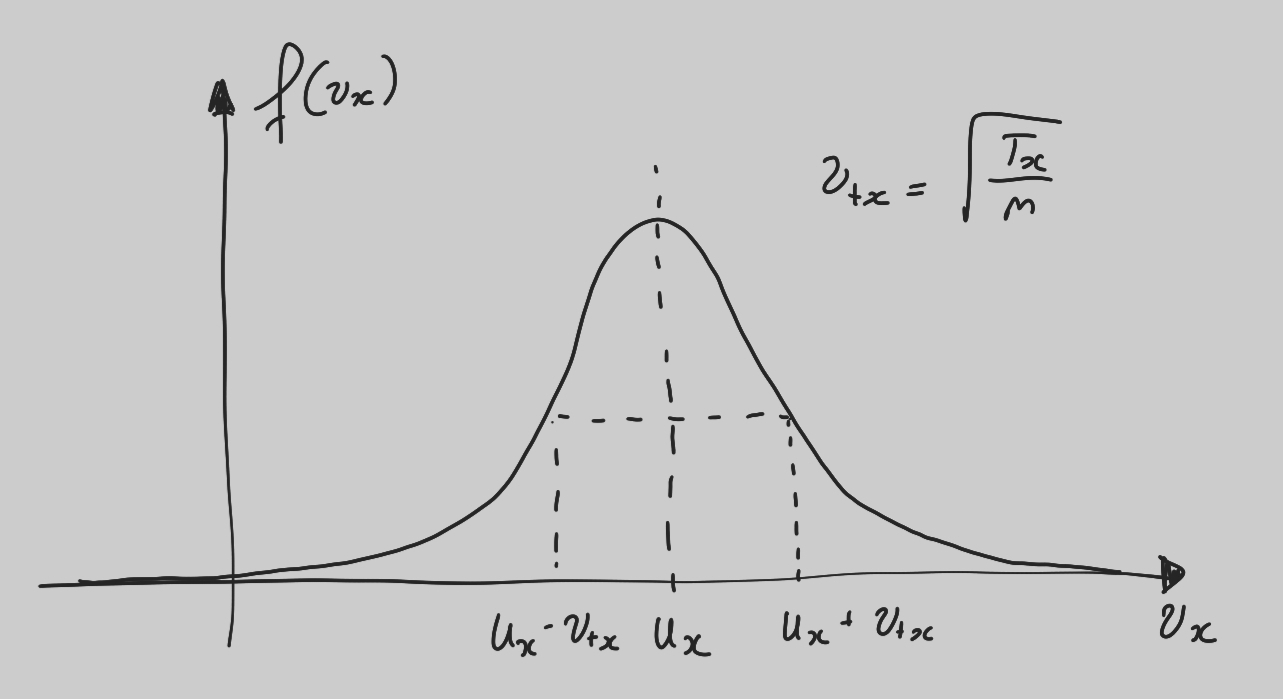
\includegraphics[width=0.8\textwidth]{5140_hw1_p1c.jpg}
    \end{figure}
\end{solution}

\end{problem}


\begin{problem}{2}[Vlasov Equation]

As done in class, let particle $n$ of a given species be defined as a Dirac
delta function
\begin{equation}
    \delta(\vb{X}_n(t)-\vb{x})\delta(\vb{V}_n(t)-\vb{v}) 
\end{equation}
where $\vb{X}_n(t)$ is the instantaneous position of a particle and
$\vb{V}_n(t)$ is the instantaneous velocity of the particle. The distribution
function for species $s$ can be described as
\begin{equation}\label{p2:dist_func}
    F_s(x,v,t)=\sum_n\delta(\vb{x}-\vb{X}_n(t))\delta(\vb{v}-\vb{V}_n(t)) 
\end{equation}

Derive the ``Vlasov Equation'' for the unsmoothed distribution $F$ using only
electromagnetic force.

\begin{solution}
    Given the distribution function \eqref{p2:dist_func}, we can differentiate
    with the chain rule
    \begin{align}\label{p2:F1}
        \frac{\partial F_s}{\partial t}
        &=\sum_n\qty[
            \frac{\partial\delta(\vb{x}-\vb{X}_n)}{\partial\vb{X}_n}
            \vdot\frac{\partial\vb{X}_n}{\partial t}\delta(\vb{v}-\vb{V}_n)
            +\delta(\vb{x}-\vb{X}_n)
            \frac{\partial\delta(\vb{v}-\vb{V}_n)}{\partial\vb{V}_n}\vdot\frac{\partial\vb{V}_n}{\partial
            t}
        ]\notag\\
        &=-\sum_n\qty{
            \vb{V}_n\vdot\qty[
            \frac{\partial\delta(\vb{x}-\vb{X}_n)}{\partial\vb{x}}
            \delta(\vb{v}-\vb{V}_n)]
        +\frac{\partial\vb{V}_n}{\partial t}\vdot
        \qty[\delta(\vb{x}-\vb{X}_n)\frac{\partial\delta(\vb{v}-\vb{V}_n)}{\partial\vb{v}}]
        }\notag\\
        &=-\sum_n\qty{
            \qty[
                \vb{V}_n\vdot\frac{\partial}{\partial\vb{x}}
            +\frac{\partial\vb{V}_n}{\partial t}
            \vdot\frac{\partial}{\partial\vb{v}}
            ]
            \qty[\delta(\vb{x}-\vb{X}_n)\delta(\vb{v}-\vb{V}_n)]
        }
    \end{align}
    where the velocity $\vb{V}_n=\partial\vb{X}_n/\partial t$ by definition.
    $\partial\vb{V}_n/\partial t$ follows the equation of motion
    \begin{equation}
        \frac{\partial\vb{V}_n}{\partial
        t}=\frac{q}{m}\qty(\vb{E}+\vb{V}_n\times\vb{B}) 
    \end{equation}
    Now, recall a property of the delta function for some arbitrary function 
    $f$
    \begin{equation}
        \sum_nf(\vb{x})\delta(\vb{x}-\vb{X}_n)
        =\sum_nf(\vb{X}_n)\delta(\vb{x}-\vb{X}_n)
    \end{equation}
    Then we can rewrite \eqref{p2:F1} as
    \begin{align}
        \frac{\partial F_s}{\partial t}
        &=-\qty[
            \vb{v}\vdot\frac{\partial}{\partial\vb{x}}
            +\frac{q}{m}\qty(\vb{E}+\vb{v}\times\vb{B})\vdot\frac{\partial}{\partial\vb{v}}
        ]
            \sum_n \delta(\vb{x}-\vb{X}_n)\delta(\vb{v}-\vb{V}_n)\notag\\
        &=-\vb{v}\vdot\frac{\partial F_s}{\partial\vb{x}}
        -\frac{q}{m}\qty(\vb{E}+\vb{v}\times\vb{B})\vdot\frac{\partial
        F_s}{\partial\vb{v}}
    \end{align}
    Re-arranging, we arrive at the Vlasov equation
    \begin{equation}
        \frac{\partial F_s}{\partial t} 
        +\vb{v}\vdot\frac{\partial F_s}{\partial\vb{x}}
        +\frac{q}{m}\qty(\vb{E}+\vb{v}\times\vb{B})\vdot\frac{\partial
        F_s}{\partial\vb{v}}
        =0
    \end{equation}
\end{solution}
    
\end{problem}


\begin{problem}{3}[Math Review]

We will use vector notation including cross products, curl, and divergences
quite often in this course so it is useful to be able to manipulate them.

(a) Show that: $\curl{\curl{\vb{A}}}=\grad(\div{\vb{A}})-\laplacian{\vb{A}}$

(b) Show that:
$\div{\qty(\vb{A}\times\vb{B})}=\vb{B}\vdot\qty(\curl{\vb{A}})-\vb{A}\vdot\qty(\curl{\vb{B}})$

\textit{Hint}: One method is to use the Levi-Civita symbol, $\xi_{ijk}$, where
\begin{equation}
    \xi_{ijk}=\begin{cases}
        1&(i,j,k)\in\qty{(1,2,3),(3,1,2),(2,3,1)}\\
        -1&(i,j,k)\in\qty{(3,2,1),(1,3,2),(2,3,1)}
    \end{cases}
\end{equation}

\begin{solution}
    (a) Starting from the LHS, we can show that
    \begin{align}
        \text{LHS}
        &=\qty(\partial_l\hat{\vb{e}}_l)\times
            \qty(\xi_{ijk}\hat{\vb{e}}_i\partial_jA_k)\notag\\
        &=\xi_{ijk}\partial_l\partial_jA_k\hat{\vb{e}}_l\times\hat{\vb{e}}_i
            \notag\\
        &=\xi_{ijk}\xi_{lin}\partial_l\partial_jA_k\hat{\vb{e}}_n\notag\\
        &=\xi_{jki}\xi_{nli}\partial_l\partial_jA_k\hat{\vb{e}}_n\notag\\
        &=(\delta_{jn}\delta_{kl}-\delta_{jl}\delta_{kn})\partial_l\partial_j
            A_k\hat{\vb{e}}_n\notag\\
        &=(\partial_j\hat{\vb{e}}_j)(\partial_kA_k)
            -\partial_j^2(A_k\hat{\vb{e}}_k)\notag\\
        &=\grad(\div{\vb{A}})-\laplacian{\vb{A}}
    \end{align}

    (b) Similarly, from the LHS
    \begin{align}
        \text{LHS}
        &=\qty(\partial_l\hat{\vb{e}}_l)\vdot
            \qty(\xi_{ijk}\hat{\vb{e}}_iA_jB_k)\notag\\
        &=\xi_{ijk}\partial_i(A_jB_k)\notag\\
        &=\xi_{ijk}\qty(B_k\partial_iA_j+A_j\partial_iB_k)\notag\\
        &=\xi_{kij}B_k\partial_iA_j-\xi_{jik}A_j\partial_iB_k\notag\\
        &=\vb{B}\vdot\qty(\curl{\vb{A}})-\vb{A}\vdot\qty(\curl{\vb{B}})
    \end{align}
\end{solution}

\end{problem}


\begin{problem}{4}[Quasi-neutral Plasma]

Calculate the condition of the ratio $\Delta N_c/N$ for gravity to dominate over
the electromagnetic force on a proton near a star. $N$ is the total number of
protons in the star and $\Delta N_c$ is the number of unbalanced charges. Show
that
\begin{equation}
    \frac{\Delta N_c}{N}\ll8\times10^{-37} 
\end{equation}

\begin{solution}
    The gravitational force exerted on a proton with mass $m$ by a cluster of
    $N$ protons in a star with mass $M=Nm$ at a distance $r$ (assuming
    $r\gg\overline{d}$ where $\overline{d}$ is the mean distance among protons
    in the star) is
    \begin{equation}\label{p4:Fg}
        F_G=\frac{GNm^2}{r^2} 
    \end{equation}
    With a number $\Delta N_c$ of unbalanced charge, the electrostatic force on
    the proton at a distance $r$ is
    \begin{equation}\label{p4:Fe}
        F_E=\frac{1}{4\pi\epsilon_0}\frac{\Delta N_ce^2}{r^2} 
    \end{equation}
    The attractive gravitational force \eqref{p4:Fg} dominates the repulsive
    electrostatic force \eqref{p4:Fe} when $F_G\gg F_E$, or in other words,
    \begin{equation}
        \frac{\Delta
        N_c}{N}\ll\frac{4\pi\epsilon_0Gm^2}{e^2}\approx8\times10^{-37} 
    \end{equation}
\end{solution}
    
\end{problem}


\begin{problem}{5}[Debye Shielding]
    
(a) Consider a conducting sphere of radius $a$ and charge $Q$ that is immersed
in a collisionless, Maxwellian plasma that has density $n_0$, $T_i=0$, but
finite $T_e$. Let $\vb{B}=\vb{0}$. Solve the time-independent electron momentum
equation
\begin{equation}\label{p5:electron_momentum}
    eEn_e+\gamma T_e\frac{\partial n_e}{\partial r}=0 
\end{equation}
to show that the isothermal equilibrium $(\gamma=1)$ electron density can be
expressed as
\begin{equation}\label{p5:ne}
    n_e=n_0e^{e\phi/T_e},\qquad r>a 
\end{equation}

(b) Let the potential at the sphere be $\phi_0$. In the limit $\phi_0\ll T_e$,
derive the potential $\phi$ as a function of $r$ in spherical coordinates.
Express your answer in terms of $r,a,\phi_0$, and $\lambda_D$.

\begin{solution}
    (a) Assume the electron density is given by \eqref{p5:ne}, then
    \begin{equation}
        \frac{\partial n_e}{\partial
        r}=\frac{e}{T_e}\frac{\partial\phi}{\partial r}n_e
        =-\frac{eE}{T_e}n_e
    \end{equation}
    where $E=-\partial\phi/\partial r$ when $\vb{B}=\vb{0}$. This is nothing but
    \eqref{p5:electron_momentum} in isothermal equilibrium ($\gamma=1$).

    (b) When $\phi_0\ll T_e$, we can write $n_e\approx n_0(1+e\phi/T_e)$ and
    Poisson equation becomes
    \begin{equation}\label{p5:poisson}
        \laplacian\phi
        =\frac1{r^2}\frac{\partial}{\partial r}
            \qty(r^2\frac{\partial\phi}{\partial r})
        =-\frac{e(n_i-n_e)}{\epsilon_0}
        \approx-\frac{en_0}{\epsilon_0}\qty[1-\qty(1+\frac{e\phi}{T_e})]
        =\frac{n_0e^2}{\epsilon_0T_e}\phi
        =\frac{\phi}{\lambda_D^2}
    \end{equation}
    where $\lambda_D$ is the Debye length. A guess to the solution for this is
    \begin{equation}
        \phi=C\frac{e^{-kr}}{r} 
    \end{equation}
    Differentiating, we can write
    \begin{equation}\label{p5:diff}
        \laplacian\phi=-\frac{C}{r^2}\frac{\partial}{\partial r}
            \qty[(kr+1)e^{-kr}]
            =Ck^2\frac{e^{-kr}}{r}=k^2\phi
    \end{equation}
    From \eqref{p5:poisson} and \eqref{p5:diff}, $k=1/\lambda_D$. Now,
    $\phi=\phi_0$ when $r=a$. Thus,
    \begin{equation}
        C\frac{e^{-a/\lambda_D}}{a}=\phi_0\Rightarrow
        C=a\phi_0e^{a/\lambda_D}
    \end{equation}
    So the full solution to the Poisson equation is
    \begin{equation}
        \phi(r)=a\phi_0e^{(a-r)/\lambda_D} 
    \end{equation}
\end{solution}

\end{problem}

\end{document}

